\documentclass[10pt, a4paper]{article}
\usepackage[english]{babel}
%\usepackage[brazilian]{babel}
\usepackage[utf8]{inputenc}
% \usepackage[T1]{fontenc}
\usepackage{lipsum}

% code
\usepackage{pythonhighlight}
\renewcommand{\lstlistingname}{Anexo} % Listing->Code
\usepackage{adjustbox}

% For subfigure use
\usepackage[font=small,labelfont=bf]{caption}
\usepackage{subcaption}

% Set page size and margins
% Replace `letterpaper' with`a4paper' for UK/EU standard size
\usepackage[a4paper,top=2cm,bottom=2cm,left=2cm,right=2cm,marginparwidth=2cm]{geometry}

% tabelas
\usepackage{array}
\usepackage{tabularx}
\usepackage{booktabs}

\usepackage{float}

% Useful packages
\usepackage{amsmath}
\usepackage{enumerate}

\usepackage{graphicx}
\usepackage[colorlinks=true, allcolors=blue]{hyperref}
\usepackage{cleveref}
\newcommand{\crefrangeconjunction}{--}


\begin{document}

\def\TITLE{Homework 01}
\def\DISCIPLINE{ELE 2346 - DEEP LEARNING}
\def\PROFESSOR{Raul Queiroz Feitosa}
\def\AUTHOR{Pedro Henrique Cardoso Paulo}
\def\CONTACT{pedrorjpaulo.phcp@gmail.com}
\def\DATE{April, 2023}

\title{\textbf{\TITLE} \\ \DISCIPLINE}
\author{\AUTHOR}
\date{\DATE}

\begin{titlepage}
      \begin{center}
          \vspace*{1cm}

          \Huge
          \textbf{\TITLE}

          \vspace{0.5cm}
          \LARGE
          \DISCIPLINE

          \vspace{1.5cm}

          \textbf{\AUTHOR \\ {\tt \CONTACT}}

          \vfill
          Professor: \PROFESSOR

          \vspace{0.8cm}

          
\includegraphics[width=0.2\textwidth]{../general/puc.jpg}

          \Large
          Departamento de Engenharia Mecânica\\
          PUC-RJ Pontifícia Universidade Católica do Rio de Janeiro\\
          \DATE

      \end{center}
  \end{titlepage}

\maketitle

\section{Introduction}

\subsection{Objectives}

The main objectives of this exercice is to provide the students some experience with:

\begin{itemize}
  \item Convolutional Neural Networks (CNNs)
  \item VGG16
  \item Transfer learning
\end{itemize}

\subsection{Dataset}

The ibeans dataset is a dataset containing images of leaves classified according to their health condition. 
The images are splitted into 3 different classes (angular leaf spot, bean rust and healthy) as shown in Figure \ref{fig:examples}.

\begin{figure}[htpb]
  \centering
  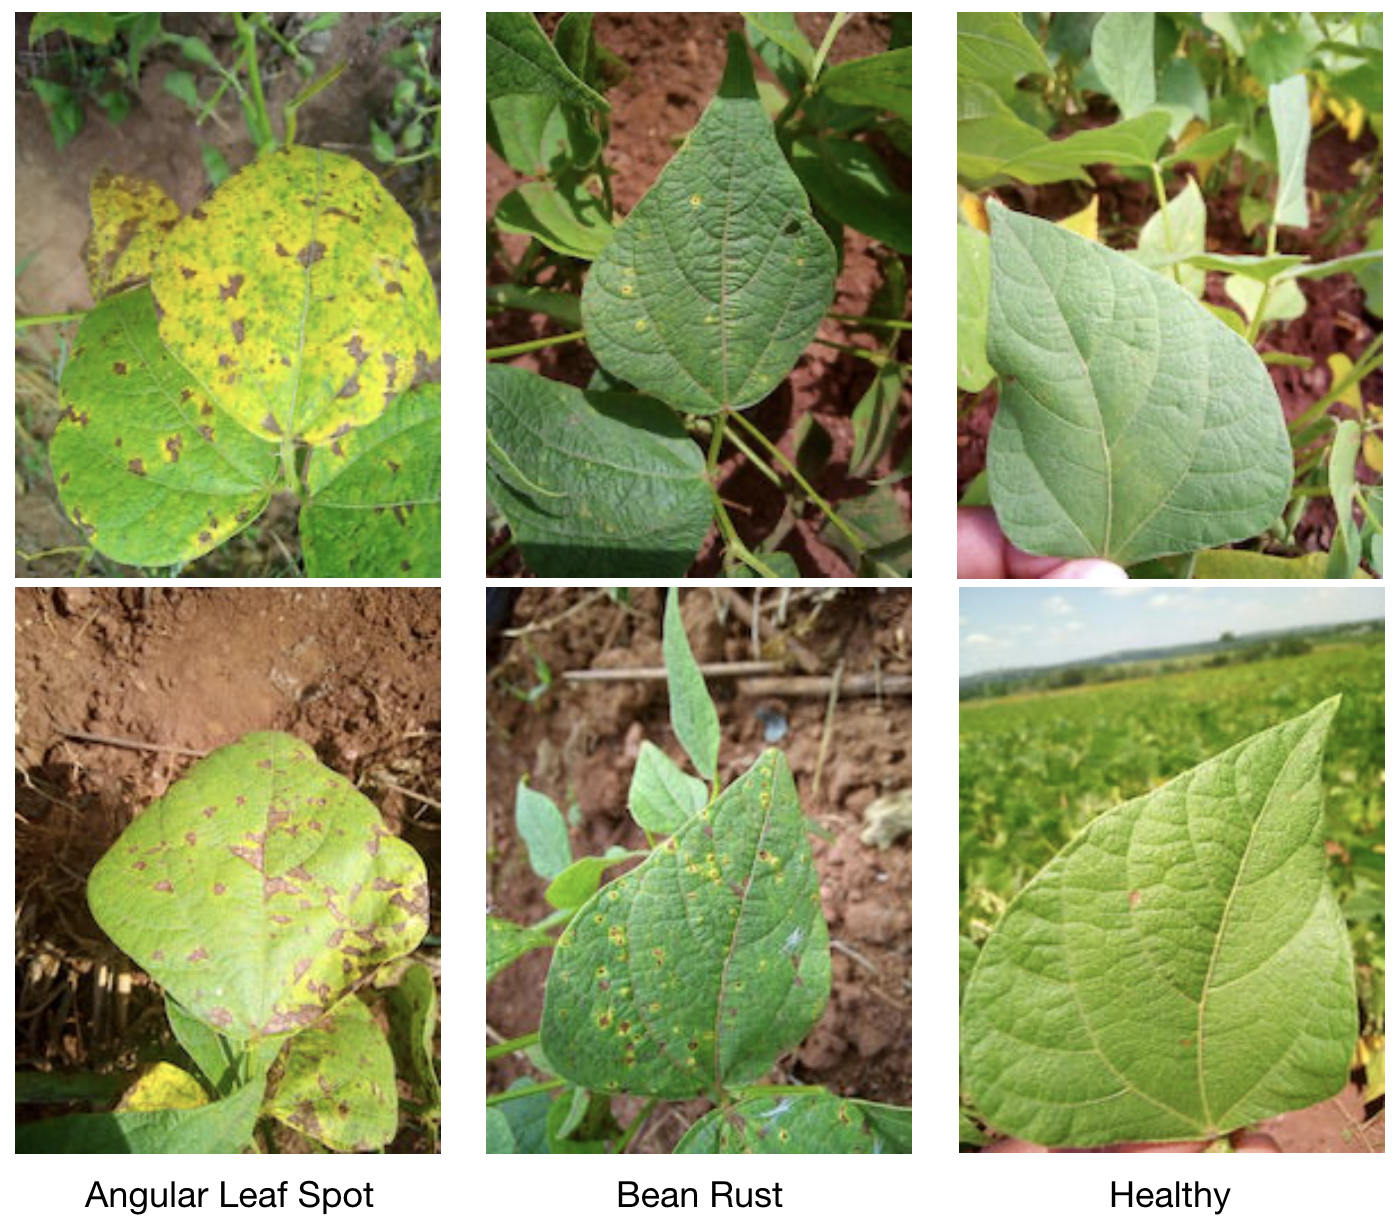
\includegraphics[width=0.8\textwidth]{images/bean-example-data.png}
  \caption{Dataset examples}
  \label{fig:examples}
\end{figure}

Since the dataset consists of images of leaves, it is possible to affirm that operations such as rotation, reflection and zooming of the image should
generate a new image with the same end label as the original one. This kind of data augmentation techniques are useful to make the network more robust
and also provide a larger dataset for the final trainning, which is useful for deep learning application. In this exercice, the same data augmentation
pipeline proposed for the in class exercice will be used.

\subsection{Exercice}

The main objective of this homework is to create a Classifier for the ibeans dataset using a VGG16 CNN model as a base. Three cases should be evaluated
for this study:

\begin{enumerate}
  \item Training from scratch: Use the VGG16 model with no prior training, remove the latest layer (prediction layer) and add a classifier. Train the model from scratch and evaluate\label{item:1}
  \item Using pre-trained network as feature extractor: Use the same model of \ref{item:1}, but with the VGG16 model pre-trained on ImageNet. Freeze all layers of ResNet50, train and evaluate the model\label{item:2}
  \item Fine-tuning the latest layers: take a pre-trained VGG16 model, unfreeze the last blocks acording to the following:\label{item:3}
  \begin{enumerate}[a]
    \item Unfreeze the last convolutional blocks (from {\tt block5\_conv1}), train and evaluate the model\label{item:3a}
    \item Unfreeze the last convolutional blocks (from {\tt block4\_conv1}), train and evaluate the model\label{item:3b}
    \item Unfreeze all convolutional blocks, train and evaluate the model\label{item:3c}
  \end{enumerate}
\end{enumerate}

Figure \ref{fig:exercice} shows an schematic of the three case studies listed above. It is worth noticing that, since the hyperparameters for the classifier should be
the same for all three cases, the choice of hyperparameters will also be a part of this study.

\begin{figure}[htpb]
  \centering
  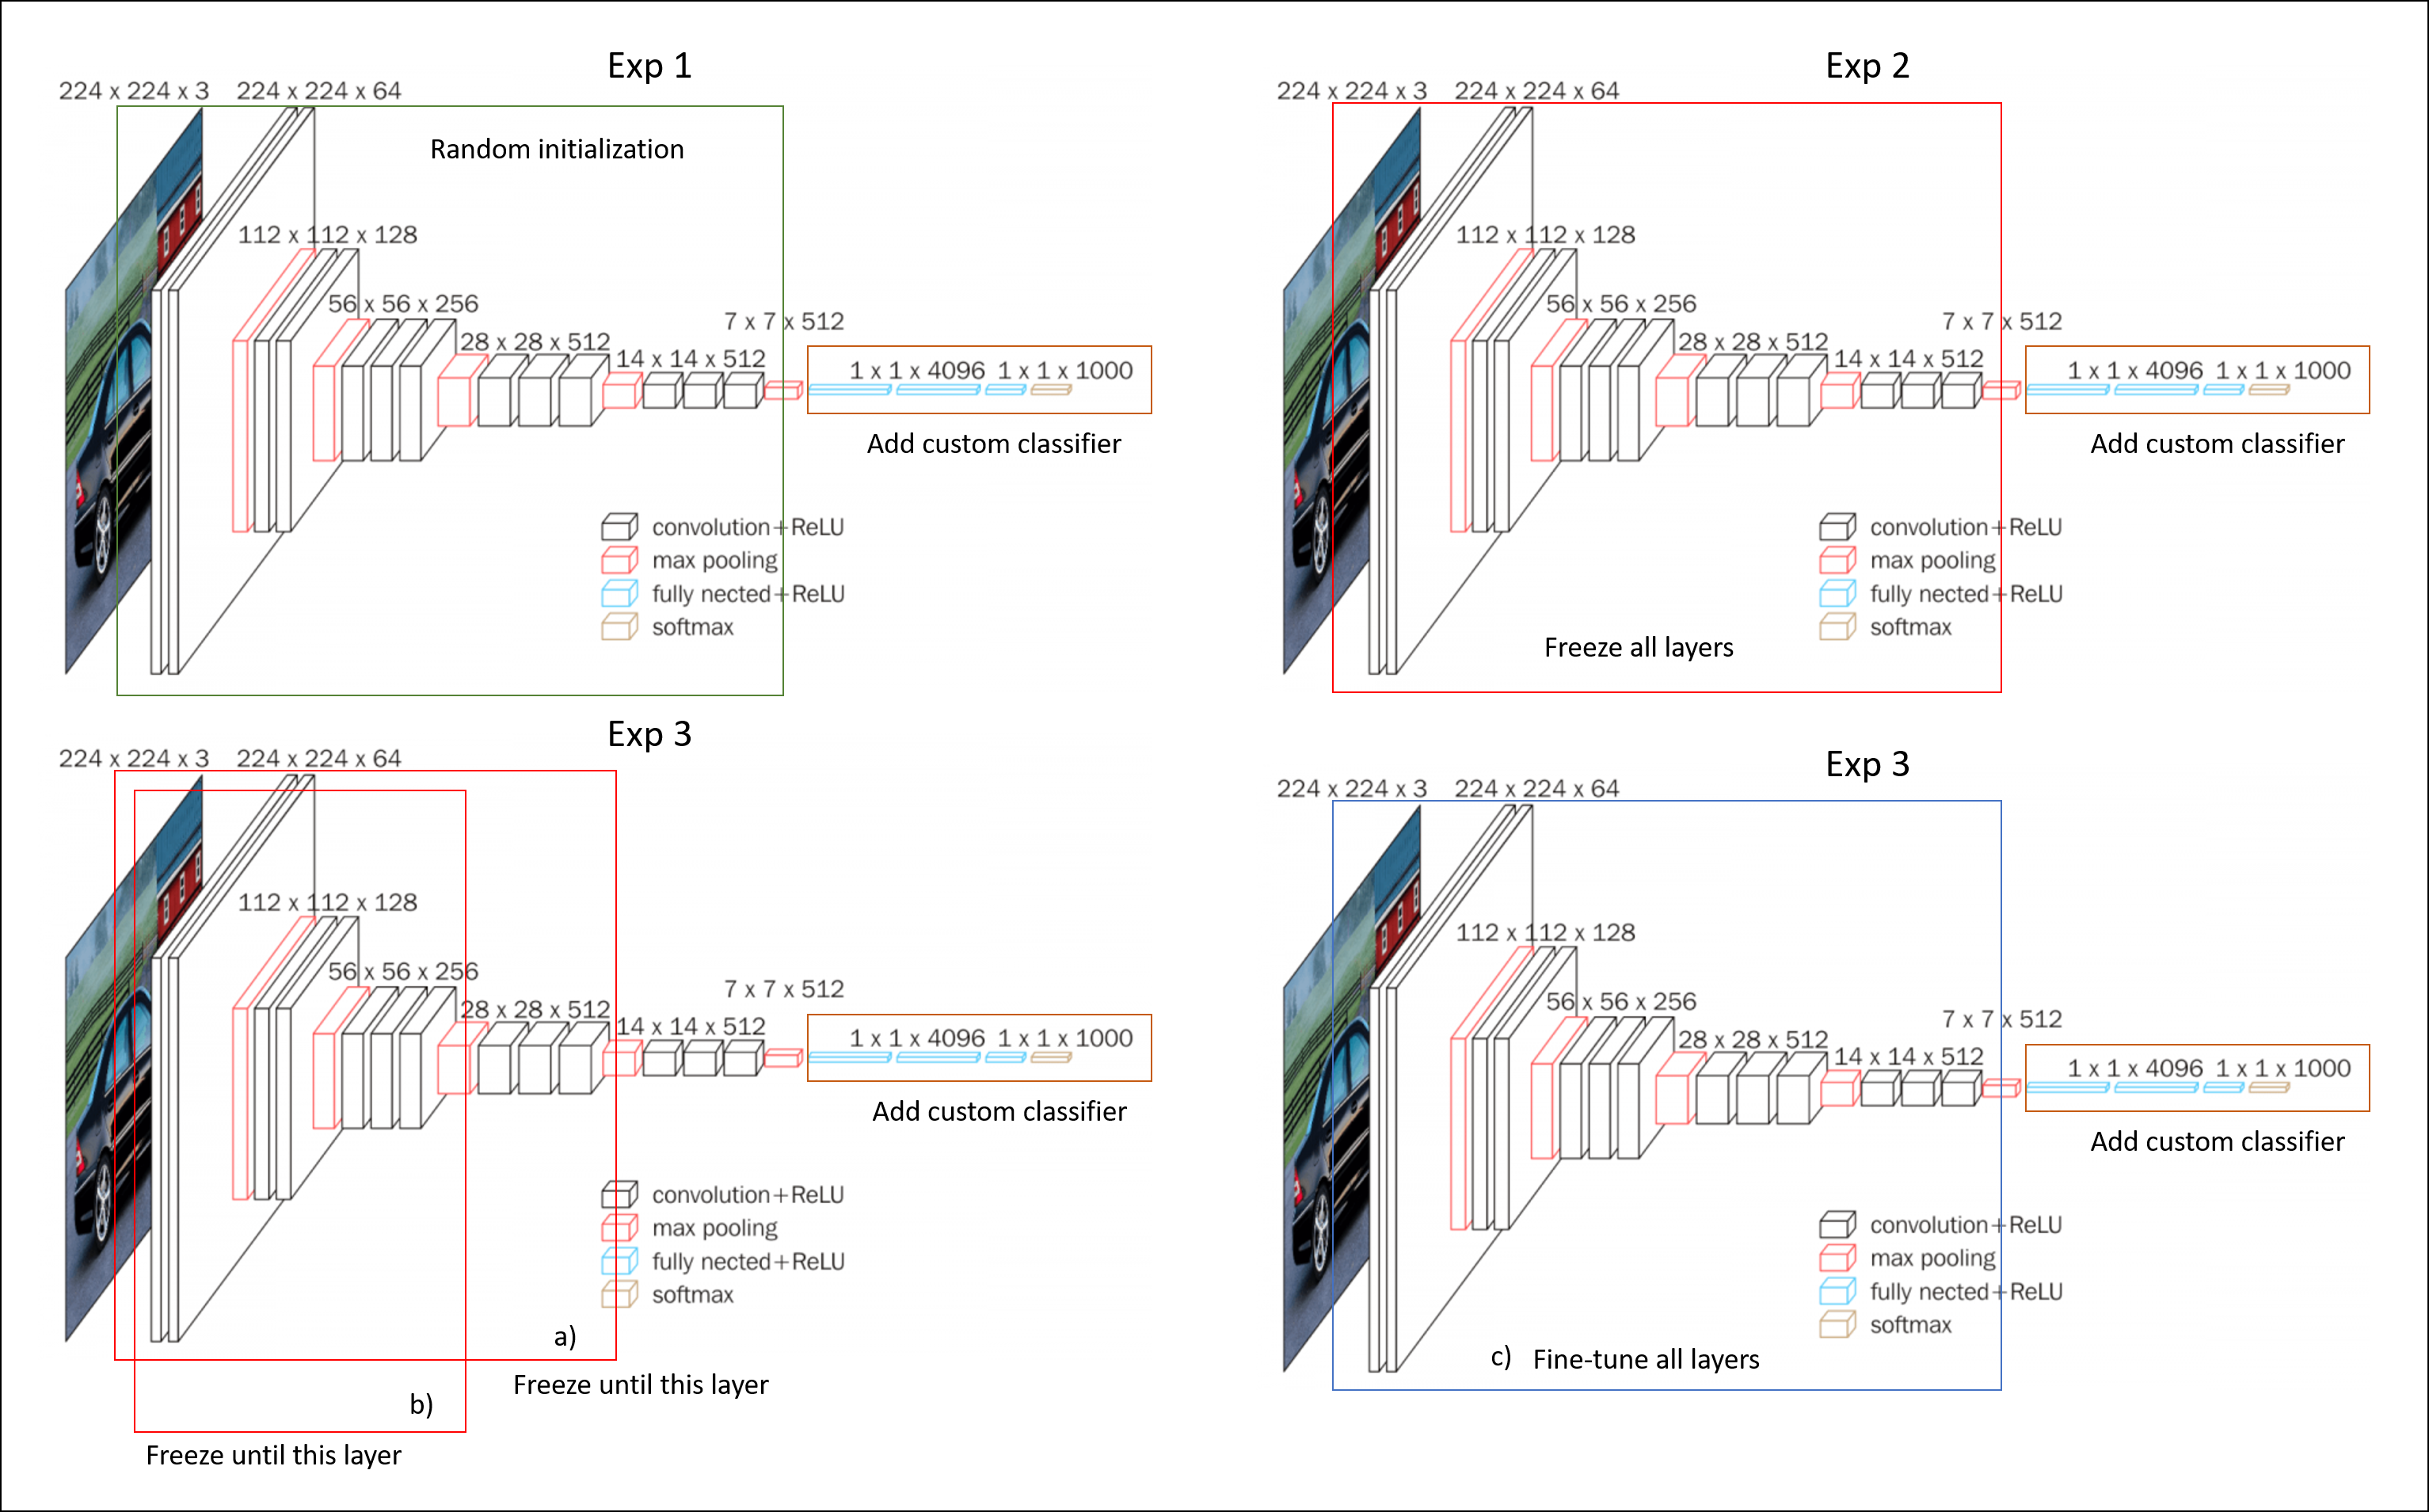
\includegraphics[width=0.8\textwidth]{images/exercice.png}
  \caption{Exercices summary}
  \label{fig:exercice}
\end{figure}

Some differences should also be noticed when comparing this homework with the practical exercice performed in class about transfer learning. First, the homework dataset
is a multi-class case, so the output layer has to be converted to a softmax-activated, 3-neuron layer. The loss and accuracy metrics used also hat to be replaced to the 
multi-class compatible {\tt CategoricalCrossentropy} and {\tt CategoricalAccuracy}, respectively. 

The multi-class nature of the problem also impacted the loading of the dataset since the problem demanded a one-hot encoding of the label in order to be compatible with the new output layer proposed. 
An example of the updated data-reading routine can be seen in the code below, where the train dataset is loaded:

\begin{python}
#Loading train
_URL = 'https://storage.googleapis.com/ibeans/train.zip'
path_to_zip = tf.keras.utils.get_file(os.path.basename(_URL), origin=_URL, extract=True)
print(path_to_zip)
train_dir = os.path.join(os.path.dirname(path_to_zip),'train')
BATCH_SIZE = 32
IMG_SIZE = (224, 224)

train_dataset = tf.keras.utils.image_dataset_from_directory(train_dir,
                                                            #Here we perform the encoding
                                                            label_mode='categorical', 
                                                            shuffle=True,
                                                            seed=1337,
                                                            batch_size=BATCH_SIZE,
                                                            image_size=IMG_SIZE)
\end{python}

\section{Results and discussions}

\subsection{Colab Notebook}

All the code, examples and tests made are documented on the following Colab Notebooks. 
The second notebook is a copy of the first created only to exercice the plot of confusion matrixes in Colab.

\begin{itemize}
  \item \href{https://colab.research.google.com/drive/1vbsj_MysbOn23sX-VEfPNyZsClUPHzFQ?usp=sharing}{Link to the Colab Notebook}
  \item \href{https://colab.research.google.com/drive/1xBnmJjsY1vJki0OXt7i3fqnDc0oXuTGr?usp=sharing}{Link to the Colab Notebook (only Confusion Matrix plots)}
\end{itemize}

\subsection{Hyperparameter selection}

The overall implemented classifier will be based on the one used in the classrom example and will be composed of:

\begin{itemize}
  \item A new {\tt Input} layer with the expected image shape
  \item The VGG16 model imported or initialized with random values
  \item A {\tt GlobalAveragePooling2D} layer to take the average of the VGG16 output channels
  \item An optional {\tt Dense} layer with {\tt "relu"} activation
  \item An output {\tt Dense} layer with 3 neurons and {\tt "softmax"} activation
\end{itemize}

The trainning will be performed in 50 epochs using the {\tt Adam} optimizer and {\tt CategoricalCrossentropy} loss.
The base learning rate will be assumed as $0.0001$, as in the classrom example.

The main hyperparameters tuned in this study were the number of nerons on the hidden layer of the classifier. 
For the hyperparameter selection, the case described in exercice \ref{item:1} was used as a base. An architecture 
with no hidden layer, an architecture with 32 neurons on the hidden layer and one with 64 neurons were tested, and 
the results are reported in table \ref{tab:hp_search}.

\begin{table}[htpb]
  \centering
  \begin{tabular}{l|c|c|c|}
    %\hline
                            & train acc  & val acc  & test acc\\
    \hline
    No hidden layer         & 92.07\%    & 95.49\%  & 89.84\% \\
    32 neurons hidden layer & 94.00\%    & 94.74\%  & 92.19\% \\
    64 neurons hidden layer & 91.88\%    & 93.23\%  & 89.06\% \\
    \hline
  \end{tabular}
  \caption{Hyperparameter test results}
  \label{tab:hp_search}
\end{table}

Based on this results, it is possible to conclude that the hidden layer with 32 neurons was the best choice, having good overall accuracies and a lower
difference in performance between train, test and validation datasets. In the Colab Notebook some tests with different learning rates were performed, but
the overall conclusion was that the initial proposed learning rate of $0.0001$ was the most adequate.

\newpage

\subsection{Exercice \ref{item:1}}

The global results of loss and accuracy for the train and validation datasets for the exercice \ref{item:1} are shown in Figure \ref{fig:e1} for the best architecture selected 
in the hyperparameter selection study performed. The evolution of the metrics are shown along the epochs of the trainning.

\begin{figure}[htpb]
  \centering
  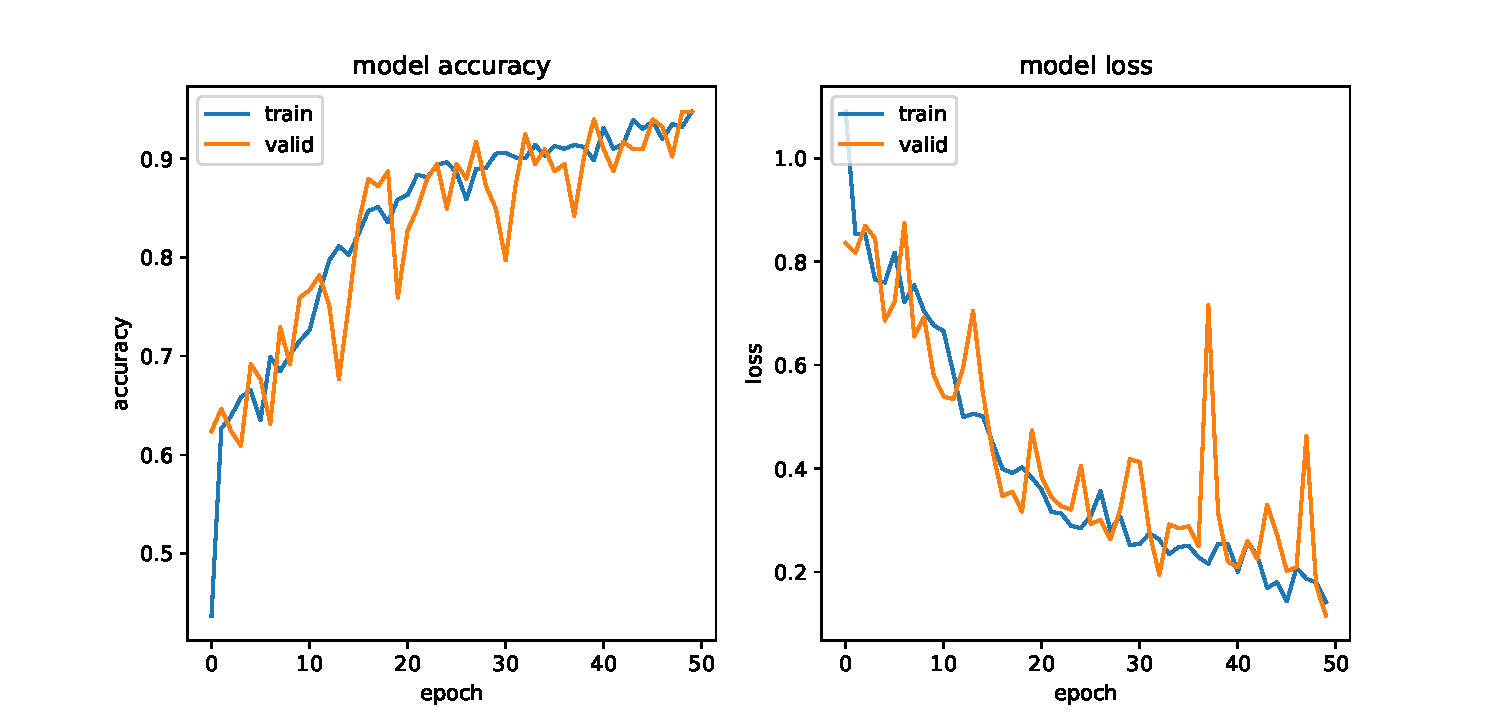
\includegraphics[width=0.8\textwidth]{images/1.2.pdf}
  \caption{Results for exercice \ref{item:1}}
  \label{fig:e1}
\end{figure}

\subsection{Exercice \ref{item:2}}

The global results of loss and accuracy for the train and validation datasets for the exercice \ref{item:2} are shown in Figure \ref{fig:e2} for the best architecture selected 
in the hyperparameter selection study performed. The evolution of the metrics are shown along the epochs of the trainning.

\begin{figure}[htpb]
  \centering
  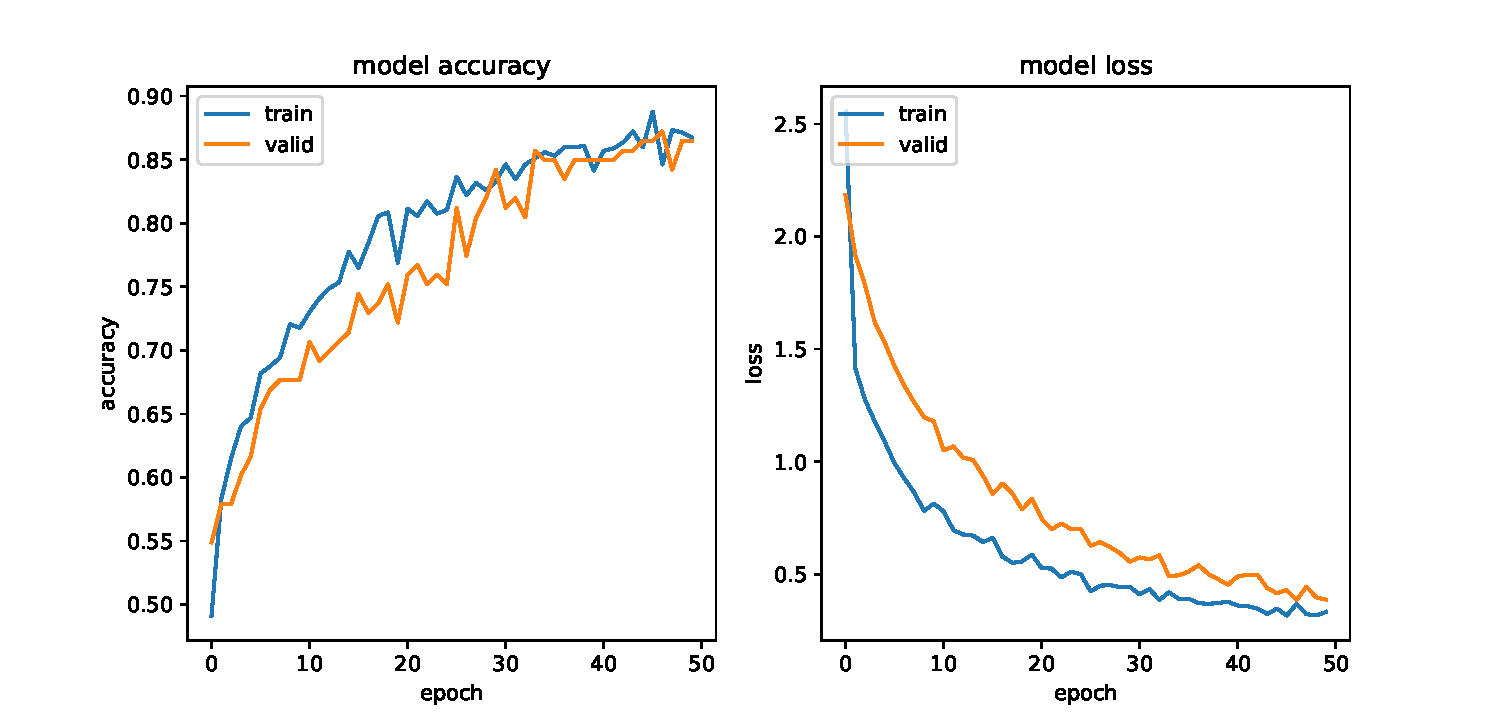
\includegraphics[width=0.8\textwidth]{images/2.pdf}
  \caption{Results for exercice \ref{item:2}}
  \label{fig:e2}
\end{figure}

\newpage

\subsection{Exercice \ref{item:3}}

\subsubsection{Item \ref{item:3a}}

The global results of loss and accuracy for the train and validation datasets for the exercice \ref{item:3a} are shown in Figure \ref{fig:e3a} for the best architecture selected 
in the hyperparameter selection study performed. The evolution of the metrics are shown along the epochs of the trainning.

\begin{figure}[htpb]
  \centering
  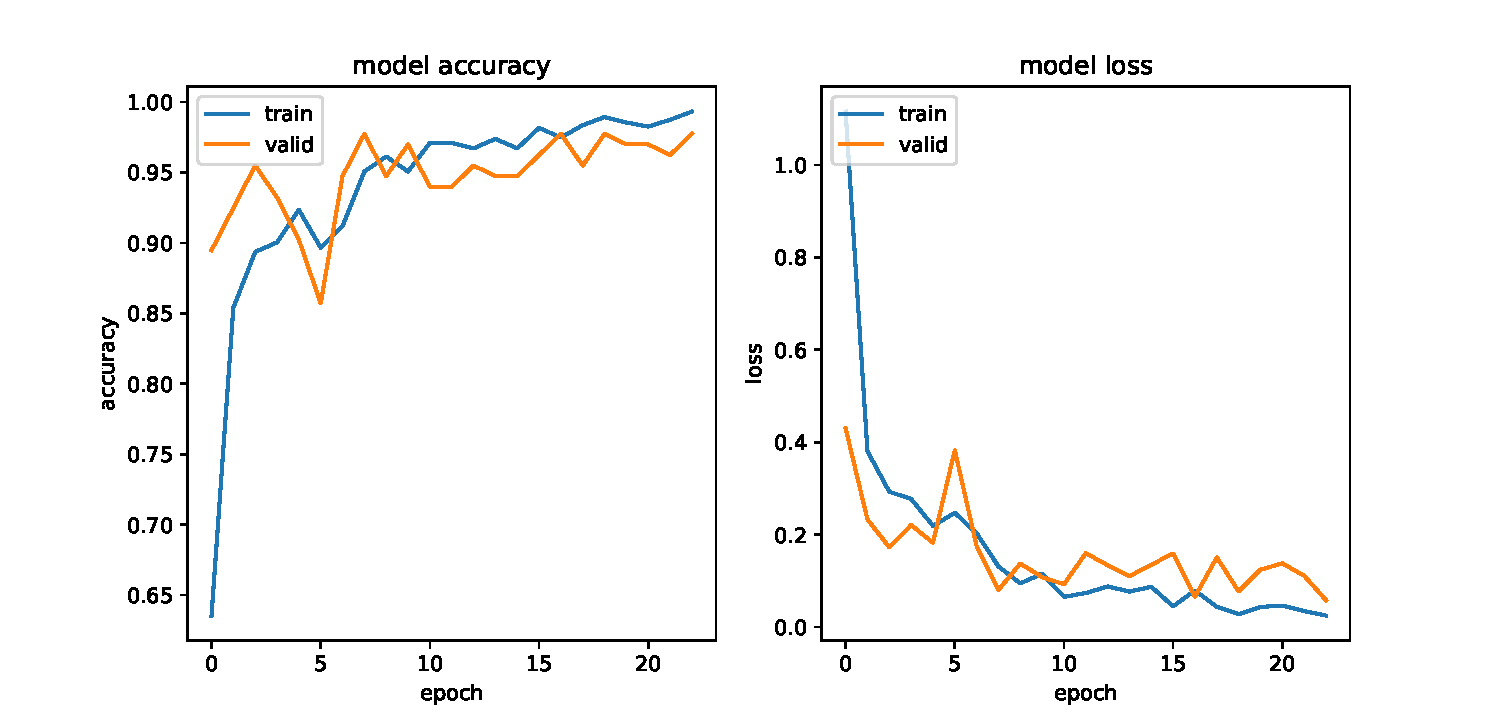
\includegraphics[width=0.8\textwidth]{images/3.a.pdf}
  \caption{Results for exercice \ref{item:3a}}
  \label{fig:e3a}
\end{figure}

\subsubsection{Item \ref{item:3b}}

The global results of loss and accuracy for the train and validation datasets for the exercice \ref{item:3b} are shown in Figure \ref{fig:e3b} for the best architecture selected 
in the hyperparameter selection study performed. The evolution of the metrics are shown along the epochs of the trainning.

\begin{figure}[htpb]
  \centering
  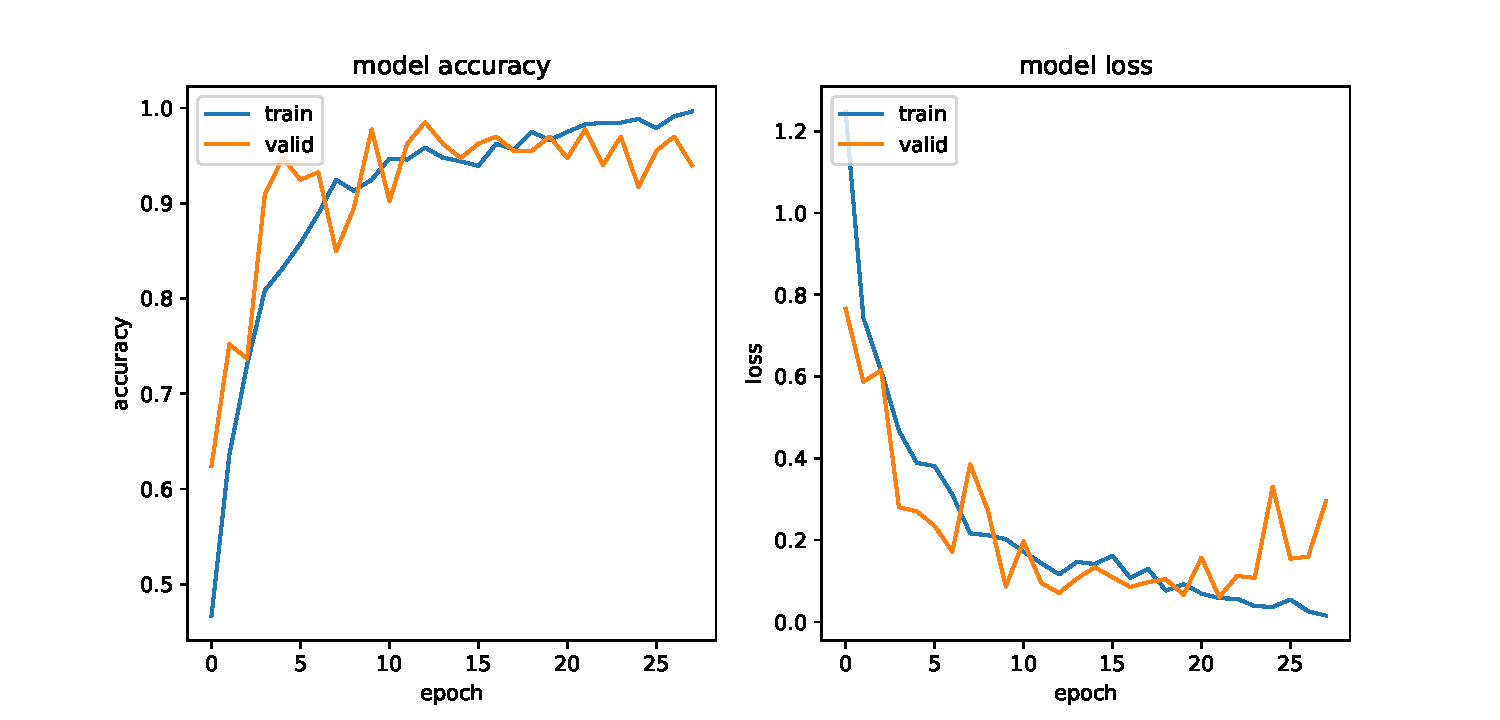
\includegraphics[width=0.8\textwidth]{images/3.b.pdf}
  \caption{Results for exercice \ref{item:3b}}
  \label{fig:e3b}
\end{figure}

\subsubsection{Item \ref{item:3c}}

The global results of loss and accuracy for the train and validation datasets for the exercice \ref{item:3c} are shown in Figure \ref{fig:e3c} for the best architecture selected 
in the hyperparameter selection study performed. The evolution of the metrics are shown along the epochs of the trainning.

\begin{figure}[htpb]
  \centering
  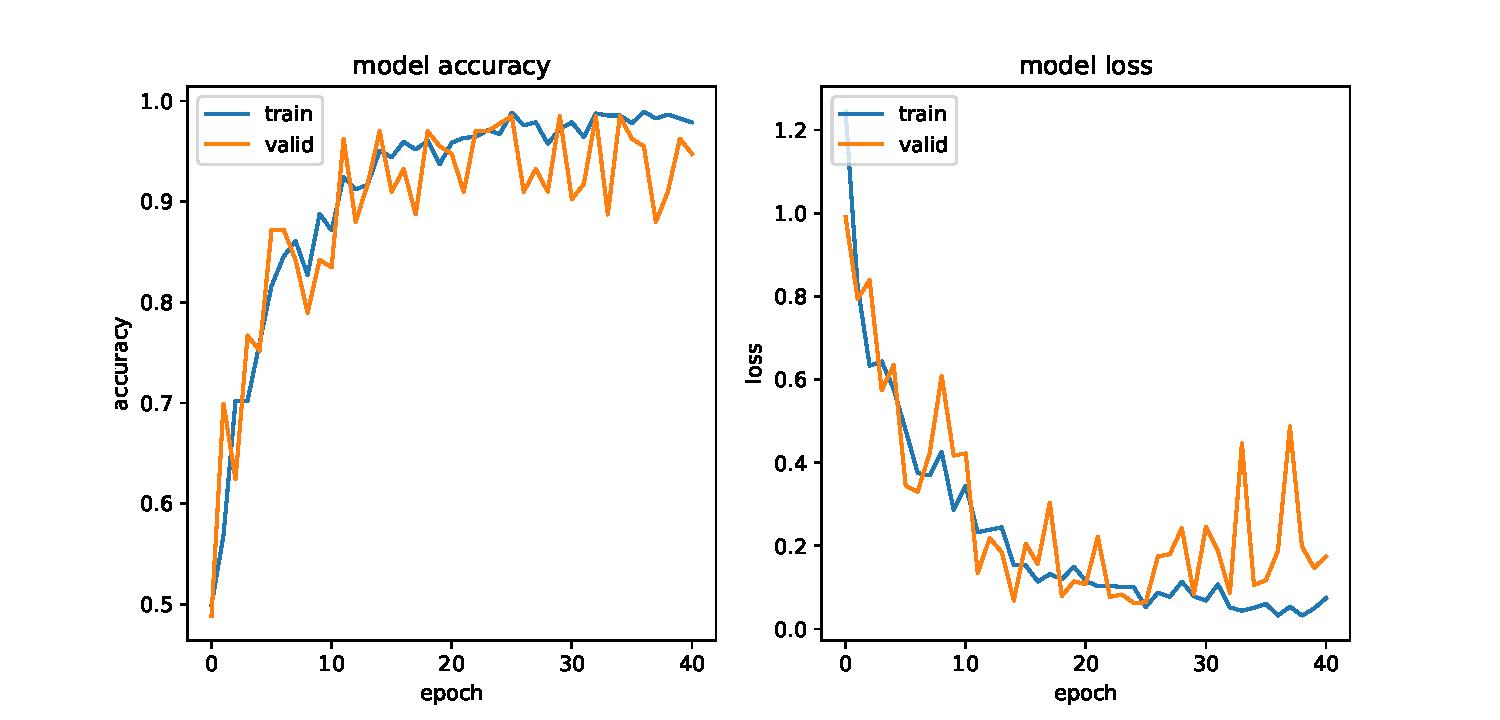
\includegraphics[width=0.8\textwidth]{images/3.c.pdf}
  \caption{Results for exercice \ref{item:3c}}
  \label{fig:e3c}
\end{figure}

\subsection{Results Summary and Conclusions}

The results summary can be seen in Table \ref{tab:results_summ}. As a general rule, it is possible to see that, while cases that have more patameters to tune such as
case \ref{item:1} and case \ref{item:2} tend to have a great difference between the train and test performance (a sign of overfitting), cases with less hyperparameters
to tune such as \ref{item:2} and \ref{item:3a} do not suffer form the same issue, having closer performences tin the train and test results. Also it is worth noticing
that the use of the ImageNet weights as the initial weights for our problem allowed lower trainning times, specially when trainning the whole network. It is also worth
mentioning that, while the use of the ImageNet weights provide a good first guess for our study, some fine-tuning of the convolutional layers is needed in order to 
obtain a performance that can be compared with trainning the whole nwtwork, with little to no loss in efficiency and even a performance increase thanks to the early stop condition
adopted.

%\footnotetext{As mentioned before, the Colab Notebook execution varies from run to run, so it is possible that}

\begin{table}[htpb]
  \centering
  \begin{tabular}{l|c|c|c|c|c|c|c|}
    Exp             &	train acc	       & train loss	    & val acc  & val loss	 & test acc	 & test loss & training time \\
    \hline
    \ref{item:1}    & 94.00\%          & 0.159551       & 94.74\%  & 0.174357  & 92.19\%   & 0.229864  & 14 min        \\
    \ref{item:2}    & 87.43\%          & 0.329751       & 92.48\%  & 0.233386  & 85.94\%   & 0.390936  & 06 min        \\
    \ref{item:3a}   & 98.26\%          & 0.055598       & 98.50\%  & 0.056195  & 96.09\%   & 0.112185  & 03 min        \\
    \ref{item:3b}   & 95.84\%          & 0.121377       & 96.24\%  & 0.082859  & 91.41\%   & 0.176876  & 04 min        \\
    \ref{item:3c}   & 97.97\%          & 0.052710       & 98.50\%  & 0.064117  & 93.75\%   & 0.230505  & 11 min        \\
    \hline
  \end{tabular}
  \caption{Results summary}
  \label{tab:results_summ}
\end{table}

Considering all the results and comments, the case \ref{item:3a} can be considered the best strategy for the current dataset since it presented good accuracy, low discrepancy in 
train and test performance and an overall low training time. The results per class can also be seen in Figure \ref{fig:conf_matrix}, where we can notice that all classes
are well-represented by the model, with most of the misclassifications ocurring between unhealthy leaves, specially {\tt bean\_rust}.

\begin{figure}[htpb]
  \centering
  \begin{subfigure}[b]{0.32\textwidth}
      \centering
      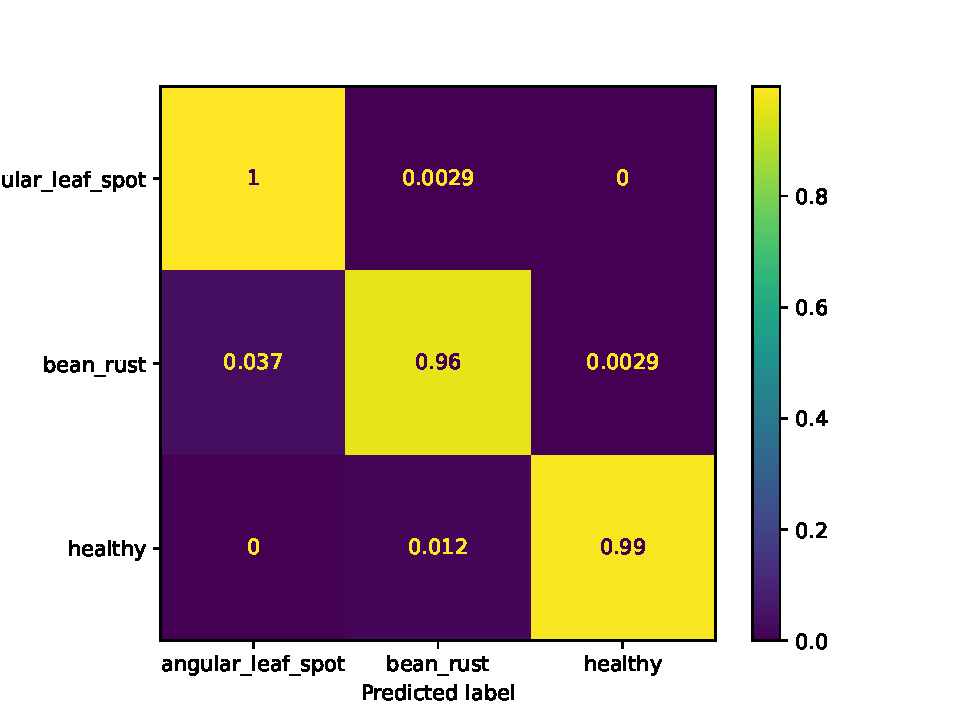
\includegraphics[width=\textwidth]{images/cm_train.pdf}
      \caption{Train set}
      \label{fig:cm_train}
  \end{subfigure}
  \hfill
  \begin{subfigure}[b]{0.32\textwidth}
      \centering
      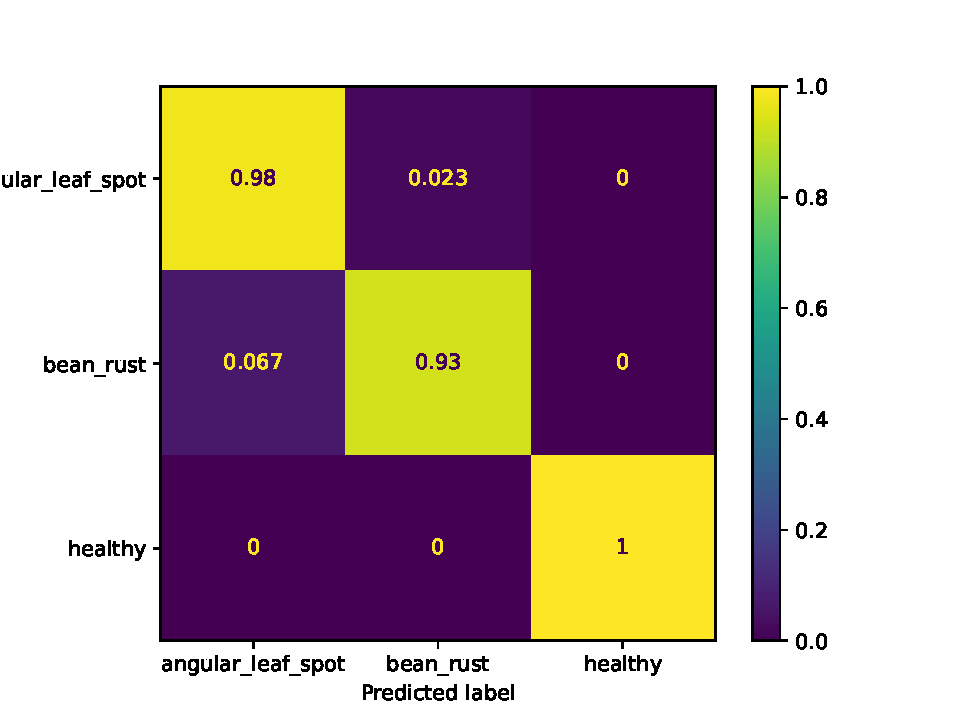
\includegraphics[width=\textwidth]{images/cm_val.pdf}
      \caption{Validation set}
      \label{fig:cm_val}
  \end{subfigure}
  \hfill
  \begin{subfigure}[b]{0.32\textwidth}
      \centering
      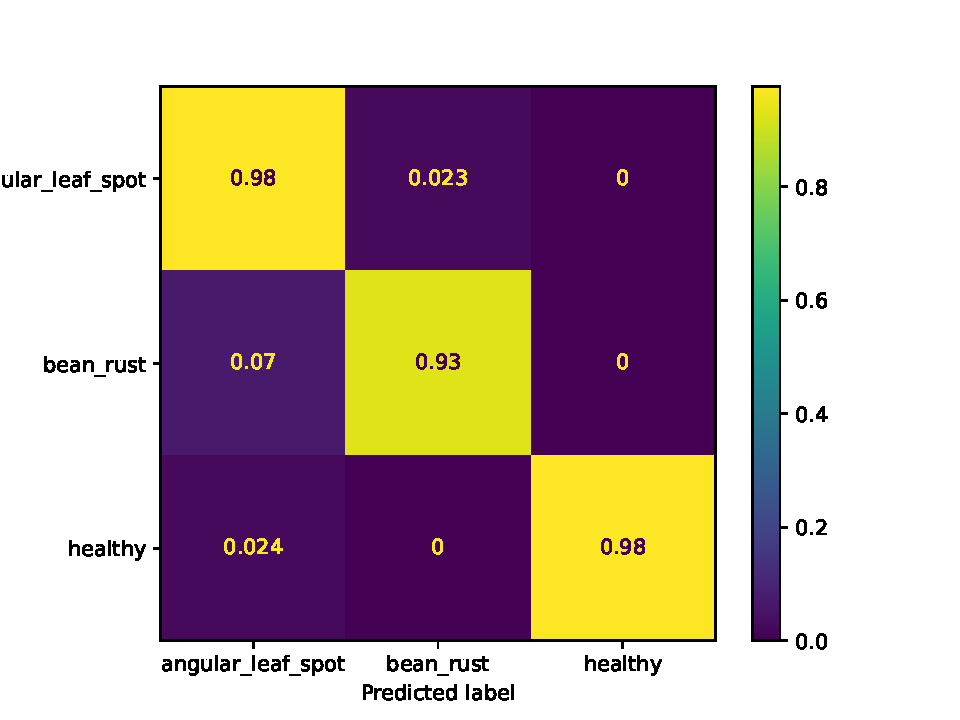
\includegraphics[width=\textwidth]{images/cm_test.pdf}
      \caption{Test set}
      \label{fig:cm_test}
  \end{subfigure}
  \caption{Confusion matrices plot for the \ref{item:3a} classifier (normalized by total real data per class)}
  \label{fig:conf_matrix}

\end{figure}


%%%%%%%%%%%%%%%%%%%%%%%%%%%%%%%%%%%%%%%%%%%%%%%%%%%

\bibliographystyle{apalike}
\bibliography{export}

\end{document}